
\chapter{Аналитическая часть}
\section[Формализация объектов синтезируемой сцены]{Формализация объектов сцены}
\label{sec:obj_formalasation}
На визуализируемой сцене могут находиться следующие объекты:
\begin{enumerate}
	\item \textbf{Точечный источник света}
	Данный источник света излучает свет во всех направлениях, интенсивность света убывает при отдалении от источника.
	Источник характеризуется:
	\begin{enumerate}[label*=\arabic*.]
		\item Положением в пространстве
		\item Интенсивностью
	\end{enumerate}
	При расчете отражений будет использоваться интенсивность источника, для расчета интенсивности пикселей. Цвет свечения будет описываться через значения RGB.
	%(TODO - в случае если останется время на физически верный расчет интенсивности то добавить постоянный, линейный и квадратичный коэффициенты)
	\item \textbf{Объекты сцены}
	
	Объектами сцены являются трехмерные примитивы:
	\begin{enumerate}[label*=\arabic*.]
		\item \textbf{Шар}
		
		Для описания шара потребуется:
		\begin{enumerate}[label*=\arabic*.]
			\item Радиус.
			\item Координаты центра.
		\end{enumerate}
		\item  \textbf{Куб}
		
		Для описания куба потребуется:
		\begin{enumerate}[label*=\arabic*.]
			\item Координаты центра.
			\item Координаты вершин относительно центра.
			\item Индексы соединенных вершин (Ребра).
		\end{enumerate}
		\item  \textbf{Конус}
		
		Для описания конуса потребуется:
		\begin{enumerate}[label*=\arabic*.]
			\item Координаты центра окружности основания конуса.
			\item Радиус основания конуса.
			\item Координата верхней точки конуса.
		\end{enumerate}
		\item  \textbf{Цилиндр}
		
		Для описания цилиндра потребуется:
		\begin{enumerate}[label*=\arabic*.]
			\item Координаты центра нижнего основания цилиндра.
			\item Координата центра верхнего основания конуса.
			\item Радиус цилиндра.
		\end{enumerate}
		Заметим, что каждый из примитивов также должен описываться своим цветом в формате RGB, а также
		коэффициентами рассеянного, диффузного, зеркального отражения. Заметим, что описанных данных достаточно для аналитического задания трехмерных тел.
		
	\end{enumerate}

	\item \textbf{Камера}
	
	В данном случае камера может описываться:
	\begin{enumerate}[label*=\arabic*.]
		\item Координатами своего положения.
		\item Вектором направления взгляда.
		\item Правым вектором пространства камеры.
		\item Верхним вектором пространства камеры.
	\end{enumerate}
	
\end{enumerate}

\section[Анализ моделей отражения]{Анализ моделей отражения}
\label{sec:reflection_models}
Свет отраженный от объекта может быть диффузным и зеркальным.
Диффузное отражение происходит, когда свет поглощается поверхностью, а затем вновь испускается, в данном случае
отражение равномерно рассеивается по всем направлениям и положение наблюдателя не имеет значения. Зеркальное отражение
происходит от внешней поверхности объекта, оно является направленным и зависит от положения наблюдателя.
Так как отражение происходит от внешней части объекта, то отраженный свет сохраняет свойства падающего, например в случае если белый свет отражается
от красного тела, отраженный свет также будет нести в себе часть красного цвета.
Для расчета интенсивности света данных отражений существует несколько моделей:
\begin{enumerate}
	\item Модель Ламберта.
	\item Модель Фонга.\cite{Rodgers}
\end{enumerate}

\subsection{Модель Ламберта}
В данной модели рассматривается диффузная составляющая отражения.

\begin{figure}[h]
	\centering
	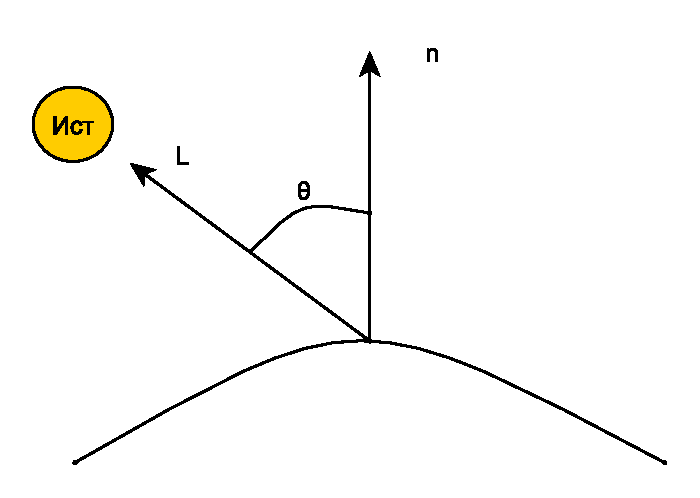
\includegraphics{lambert_model}
	\caption{Модель ламберта}
	\label{fig:lambert_model}
\end{figure}

Считается, что интенсивность отраженного света
пропорциональна косинусу угла между направлением света и нормалью к поверхности:
\begin{equation} 
	I = k_aI_a + I_lk_l\cos\theta \quad 0 \leq \theta \leq \pi/2.
	\label{eq:lambert_model}
\end{equation}
В  формуле~\ref{eq:lambert_model}:
\begin{enumerate}
	\item $k_a,k_d$ - коэффициенты рассеянного, диффузного отражения соответственно.
	\item $I_a,I_l$ - интенсивность рассеянного и диффузного отражения.
	\item $\theta$ - угол между нормалью к поверхности и направлением света.
\end{enumerate}
Заметим что значения приведенных коэффициентов лежат на отрезке от 0 до 1.

Однако интенсивность света должна убывать с увеличением расстояния от источника до объекта, эмпирически было выведено следующее соотношение:
\begin{equation} 
	I = k_aI_a + \frac{I_lk_l\cos\theta}{d + K}.
	\label{eq:lambert_model_space}
\end{equation}
В данном случае добавлены $d,K$, в случае если точка наблюдения на бесконечности, то $d$ - определяется положением объекта,
ближайшего к точке наблюдения, то есть он будет освещаться с максимальной интенсивностью источника, а дальние объекты - с уменьшенной.
Таким образом $K$ - произвольная постоянная. \cite{Rodgers}


\subsection{Модель Фонга}
Данная модель также учитывает зеркальную составляющую отражения
\begin{figure}[h]
	\centering
	\includegraphics{phong_model}
	\caption{Расчет зеркальной составляющей отражения}
	\label{fig:phong_model}
\end{figure}

Зеркальная составляющая отражения имеет следующий вид:
\begin{equation} 
	I_s = I_l\omega(i,\lambda)\cos^n \alpha.
	\label{eq:phong_model}
\end{equation}

В формуле~\ref{eq:phong_model} символы соответственно означают:
\begin{enumerate} 
	\item $\omega(i,\lambda)$ - кривая отражения, показывающая отношение зеркально отраженного света к падающему, как функцию угла падения $i$ и длинны волны $\lambda$.
	\item $\alpha$ - угол между отраженным лучом и вектором, проведенным из точки падения луча в точку наблюдения.
	\item $n$ - степень, аппроксимирующая пространственное распределение отраженного света.
	\item $I_l$ - интенсивность падающего луча.
\end{enumerate}
Функция $\omega(i,\lambda)$ сложна, так что ее заменяют константой $k_s$, получаемой экспериментально.


Таким образом формула принимает следующий вид:
\begin{equation} 
	I = k_aI_a + k_dI_{l}(\hat{n} \cdot \hat{L}) + k_s  I_{l}(\hat{S} \cdot \hat{R})^n.
\end{equation}
В данном случае косинусы вычисляются с помощью скалярного произведения нормированных векторов:
\begin{enumerate}
	\item $\hat{n}$ - вектор нормали поверхности в точке падения.
	\item $\hat{L}$ - вектор падающего луча.
	\item $\hat{S}$ - вектор наблюдения.
	\item $\hat{R}$ - вектор отражения.
\end{enumerate}
Символ $\hat{}$ означает, что данный вектор нормированный.\cite{Rodgers}




\subsection{Выбор модели отражения}
Данные модели описывают простую (локальную) модель освещения, то есть модель освещения в которой учитывается свет, попадающий в рассматриваемую точку от источника света.
Для получения отражений стоит использовать глобальную модель освещения, в которой также учитывается интенсивность света, отраженного от других поверхностей, пример описания глобальной модели излучения можно найти в секции~\ref{sec:ray_tracing}.
Заметим, что глобальная модель в случае алгоритма Уиттеда освещения использует идею модели Фонга (см.~\ref{eq:intensivity}).






\section[Анализ алгоритмов создания отражений]{Анализ алгоритмов визуализации}

Для начала рассмотрим пример отражения лучей:

\begin{figure}[H]
	\centering
	\includegraphics{global_model_light}
	\caption{Пример трассировки луча}
	\label{fig:global_model_light}
\end{figure} 

Заметим что на рисунке~\ref{fig:global_model_light}  призма, загороженная от наблюдателя параллелепипедом, становится видимой из-за отражения в сфере.
Точка 5 видима, так как отражается от обратной стороны параллелепипеда в точке 4 к точке 3 на сфере, а затем к наблюдателю.
Таким образом, при создании глобальной модели освещения, алгоритмы, основанные на удалении невидимых поверхностей не будут давать изображения необходимого качества.
Таким образом глобальная модель освещения является частью алгоритмов выделения видимых поверхностей путем трассировки лучей\cite{Rodgers}


При построении реалистичного изображения необходимо с полированными поверхностями необходимо визуализировать отражения света от тел.
Существуют множество подходов для создания реалистичных изображений:
\begin{enumerate}
	\item Трассировка световых лучей (англ. Ray tracing)
	\item Отображения отражений (англ. Reflection mapping)
	\item Трассировка лучей в пространстве изображения (англ. Screen-space reflections)
\end{enumerate}





\subsection{Алгоритм трассировки лучей}
\label{sec:ray_tracing}
\textbf{Основная идея алгоритма - симуляция физического процесса прохождения света.} \par
В реальной жизни объекты являются видимыми, в случае если они отражают свет от источника, после чего данные лучи света попадают в человеческий глаз. Аналогичная идея заложена в данном способе создания изображения - необходимо отследить движение лучей света.
Заметим, что отслеживать путь всех лучей света не стоит, так как это неэффективно, при построении изображения внимание следует уделять объектам видимыми со стороны наблюдателя.
В таком случае можно отслеживать лучи света, исходящие из точки наблюдения, т.~е. производить трассировку лучей в обратном направлении. В нашем случае лучи стоит проводить через центры пикселей изображения,
считается, что наблюдатель находится на бесконечности, из-за чего все лучи параллельны оси OZ.\cite{Rodgers,modern_ray_tracing}

\begin{figure}[h]
	\centering
	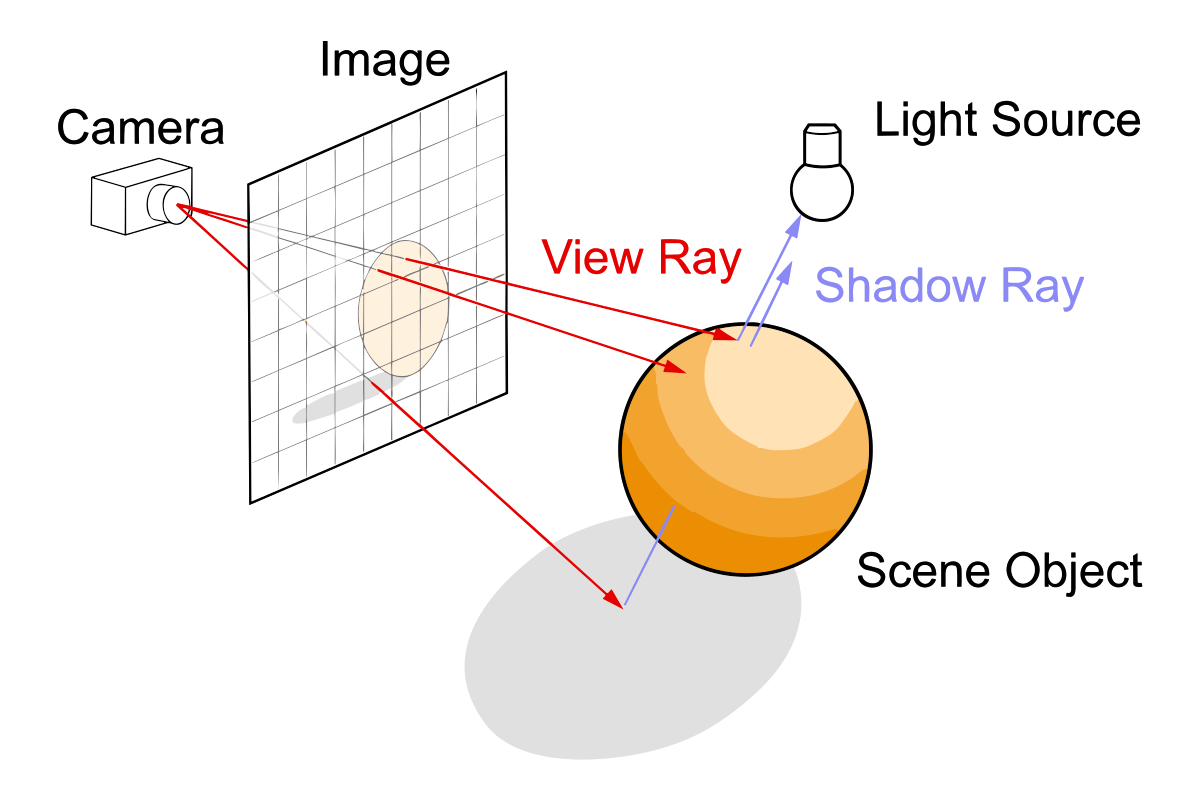
\includegraphics[scale=0.3]{ray_tracing}
	\caption{Пример трассировки луча}
	\label{fig:alg_ray_tracing}
\end{figure} 

Первые работы принадлежат Уиттеду и Кэю. Алгоритм Уиттеда более общий и часто используется.
Уиттед пользуется моделью, в которой диффузная и зеркальная составляющие отражения рассчитываются подобно локальной модели (см.~\ref{sec:reflection_models}).
Диффузное отражения одинаково во всех направлениях, так что наибольшую проблему представляет расчет зеркальных отражений.\cite{Rodgers}

\begin{figure}[h]
	\centering
	\includegraphics{global_reflections}
	\caption{Расчет зеркального отражения луча в алгоритме Уиттеда}
	\label{fig:global_reflections}
\end{figure} 

На рисунке~\ref{fig:global_reflections} луч \textbf{V} падает на поверхность в точку \textbf{Q}, после чего отражается в направлении \textbf{r} и преломляется
в направлении \textbf{p}.
В данном случае:
\begin{enumerate}
	\item $I_t$ - интенсивность света, проходящего по преломленному лучу \textbf{p}.
	\item $\eta$ - показатели преломления сред (влияют на направление преломленного луча).
	\item $\hat{S},\hat{R}$ - полученные вектора наблюдения и отражения.
	\item $\hat{L_j}$ - Вектор к источнику света $j$.

\end{enumerate}

Тогда наблюдаемая интенсивность \textbf{I} выражается формулой:
\begin{equation} 
	I = k_aI_a + k_d \sum_{j} I_{l_j}(\hat{n} \cdot \hat{L_j}) + k_s \sum_{j} I_{l_j}(\hat{S} \cdot \hat{R_j})^n + k_sI_s + k_tI_t.
	\label{eq:intensivity}
\end{equation}

В формуле~\ref{eq:intensivity} соответственно означают:
\begin{enumerate}
	\item $k_a,k_d,k_s$ - коэффициенты рассеянного, диффузного, зеркального отражения соответственно.
	\item $k_t$ - коэффициент пропускания.
	\item $n$ - степень пространственного распределения Фонга.
\end{enumerate}
В данном случае знак $ \hat{} $  означает что данный вектор нормализован.
Значения коэффициентов определяются внешней средой, свойствами материала объектов и длинной волн света
Таким образом возможно посчитать интенсивность света для отраженной и преломленной части луча.
После чего полученные вычисления необходимо выполнить еще раз для отраженного и преломленного луча и т.~д., а также сложить полученные интенсивности.
Теоретически свет может отражаться бесконечно, так что стоит ограничить число рассматриваемых отражений либо определенным числом,
либо не рассматривать лучи с интенсивностью меньше определенного значения
Таким образом данный алгоритм имеет асимптотику $O(N \cdot C \cdot 2^{K})$, где \textbf{N} - количество тел,\textbf{C} - количество испускаемых лучей,
\textbf{K} - количество рассматриваемых отражений света. \cite{Rodgers}



\textbf{Достоинства алгоритма}:
\begin{enumerate}
	\item Создание реалистичных изображений. \cite{Rodgers,modern_ray_tracing,SSR}
	\item Возможность наблюдения физических явлений, так как алгоритм симулирует поведение света в реальной жизни. \cite{Rodgers,modern_ray_tracing,SSR}
\end{enumerate}


\textbf{Недостатки алгоритма}:
\begin{enumerate}
	\item Долгое время работы. \cite{Rodgers,modern_ray_tracing,SSR}
	\item Количество требуемой памяти, так как в памяти необходимо хранить все отраженные и преломленные лучи, полученные при предыдущих расчетах. \cite{Rodgers,modern_ray_tracing,SSR}
\end{enumerate}


\subsection{Трассировка лучей в пространстве изображения}
\textbf{Основная идея алгоритма - симуляция физического процесса прохождения света, рассматривая только видимые объекты.} \par
Обычно при необходимости расчета отражений и теней уже известны объекты, которые находятся на сцене. При использовании алгоритма трассировки лучей в пространстве изображения (англ. Screen-space reflections, SSR), используется информация о имеющихся
объектов из-за чего трудозатраты на создание изображения заметно сокращаются.
Асимптотическая оценка данного алгоритма аналогична асимптотической оценке алгоритма трассировке лучей, однако в данном случае будут анализироваться только видимые объекты.\cite{SSR}

Перед началом алгоритма требуется информация для каждого пикселя:
\begin{enumerate}
	\item Координата Z наиближайшей к наблюдателю поверхности.
	\item Нормаль данной поверхности.
\end{enumerate}

\begin{figure}[H]
	\centering
	\includegraphics{SSR_data_flow.png}
	\caption{Поток данных при использовании SSR}
	\label{fig:SSR_data_flow}
\end{figure} 

До начала работы самого алгоритма необходимо подготовить данные, что происходит в два этапа:
\begin{enumerate}
	\item Геометрический проход (англ. Geometry pass).
	\item Световой проход (англ. Lightning pass).
\end{enumerate}

На картинке~\ref{fig:SSR_data_flow} используется понятие \textbf{G-buffer}, этот буфер содержит все необходимые данные для начала работы алгоритма, данные для данного буфера
будут получены после геометрического прохода. В общем случае он содержит для каждого пикселя:
\begin{enumerate}
	\item Нормали к видимым поверхностям.
	\item Значение z наиближайшей видимой фигуры.
	\item Свойства материалов, значимые для трассировки света (коэффициенты диффузного и зеркального отражения).
\end{enumerate}
При световом проходе для каждого пикселя выбираются источники, которые влияют на его интенсивность
Работа SSR аналогична работе алгоритма \textbf{Ray tracing}, однако информация о видимых объектах уже получена и будут рассматриваться только они.
Из-за этого, если часть объекта не видима то изображение будет не корректным, как, например, на картинке~\ref{fig:SSR_fail}.\cite{SSR,reflexion_types}
\begin{figure}[H]
	\centering
	\includegraphics[scale=0.4]{SSR_fail.jpg}
	\caption{Некорректный расчет отражений при использовании SSR}
	\label{fig:SSR_fail}
\end{figure} 

\textbf{Достоинства алгоритма}:
\begin{enumerate}
	\item Меньшее число трудозатрат, чем при использовании алгоритма трассировки лучей. \cite{SSR}
\end{enumerate}

\textbf{Недостатки алгоритма}:
\begin{enumerate}
	\item При наличии невидимых для наблюдателя частей объектов в отражении изображение будет некорректным. \cite{SSR}
	\item Искажение геометрии при генерации изображений. \cite{SSR}
\end{enumerate}

\subsection{Отображение отражений}
\textbf{Основная идея - создание текстуры с уже просчитанными отражениями, после чего наложить ее на зеркальный предмет} 
Для того чтобы получить текстуру, достаточно предварительно рассчитать изображения в 6 направлениях для необходимого объекта, получив кубическую карту, ее пример представлен на картинке~\ref{fig:cube_maps}.\cite{reflexion_types}
\begin{figure}[h]
	\centering
	\includegraphics[scale=0.4]{cube_maps}
	\caption{Пример кубической карты (англ. cube maps)}
	\label{fig:cube_maps}
\end{figure}

Например, для объекта~\ref{fig:cube_maps_real}, будет получена карта~\ref{fig:cube_maps_real_example}


\begin{figure}[H]
	\centering
	\includegraphics[scale=0.4]{cube_maps_real}
	\caption{Положение объекта для построения карты}
	\label{fig:cube_maps_real}
\end{figure}


\begin{figure}[H]
	\centering
	\includegraphics[scale=0.4]{cube_maps_real_example}
	\caption{Полученная кубическая карта}
	\label{fig:cube_maps_real_example}
\end{figure}


Однако динамически обновлять данную текстуру очень трудозатратно (необходимо отрисовать сцену 6 раз). Асимптотическая оценка зависит от алгоритма, выбранного для построения изображения каждой грани куба.


\textbf{Достоинства алгоритма}:
\begin{enumerate}
	\item При статических текстурах не тратится время на расчет отражений и теней. \cite{reflexion_types}
\end{enumerate}

\textbf{Недостатки алгоритма}:
\begin{enumerate}
	\item Расчет изменяющейся картинки очень трудозатратен. \cite{reflexion_types}
\end{enumerate}

\subsection{Выбор оптимального алгоритма}
При реализации отражений примитивов точность их представления играет решающую роль. Единственный алгоритм из рассмотренных, который позволяет представить максимально
реалистичное изображение - \textbf{алгоритм трассировки лучей}. Так как выбранные примитивы простые, то при использовании данного алгоритма вычислительная
сложность не будет являться критически высокой. Алгоритм  трассировки в пространстве изображения хорошо показывает себя при необходимости генерации неправдоподобных отражений, кубические карты
используются при возможности создания статических изображений, эти ограничения не позволяют их использовать при генерации реалистичных изображений.


\textbf{Выводы}

В данном разделе были проанализированы модели отражения и алгоритмы создания отражений.
Таким образом были выбраны:
\begin{enumerate}
	\item \textbf{Алгоритм создания отражений} - Алгоритм обратной трассировки лучей.
	\item \textbf{Модель отражения} - Модель отражения Фонга.
\end{enumerate}


Входными данными для полученной системы будут являться:
\begin{enumerate}
	\item Интенсивность источника.
	\item Спектральные характеристики материала примитива.
	\item Положение источника.
	\item Положение примитива.
	\item Угол поворота примитива.
\end{enumerate}